\chapter{Methods: architectures and training}
\label{chap:methods}

We compare three architectures of increasing complexity. They share the same
interface --- input a single-channel window $\mathbf{x}\in\R^{1\times 512}$,
output $K=7$ class logits --- so they are interchangeable in one training and
evaluation pipeline. This chapter covers the input pipeline
(\cref{sec:windowing}), the building blocks we use (\cref{sec:blocks}), the three
networks (\cref{sec:arch}) and the training recipe (\cref{sec:training}). We
describe only the operations the models actually use.

\section{Windowing, labelling and normalisation}
\label{sec:windowing}

\paragraph{Temporal split and windows.} To avoid leakage between overlapping
windows, the raw signal is split along time first (first $80\%$ for
train\,+\,validation, last $20\%$ for test); sliding windows of length $W=512$
are then extracted independently in each part with stride $32$ at training time.

\paragraph{Window labelling.} A window may straddle background and an event. We
label it by \emph{coverage}: if anomalous samples make up at least
$\tau_{\mathrm{cov}}=10\%$ of the window, the window takes the majority anomaly
class among them; otherwise it is \texttt{Normal} (\cref{fig:windowing}). The
$10\%$ floor keeps a window from being called anomalous on the strength of a few
boundary samples, while the abundant injection density of the benchmark
(\cref{sec:generator}) still yields many positive windows per morphology.

\begin{figure}[H]
    \centering
    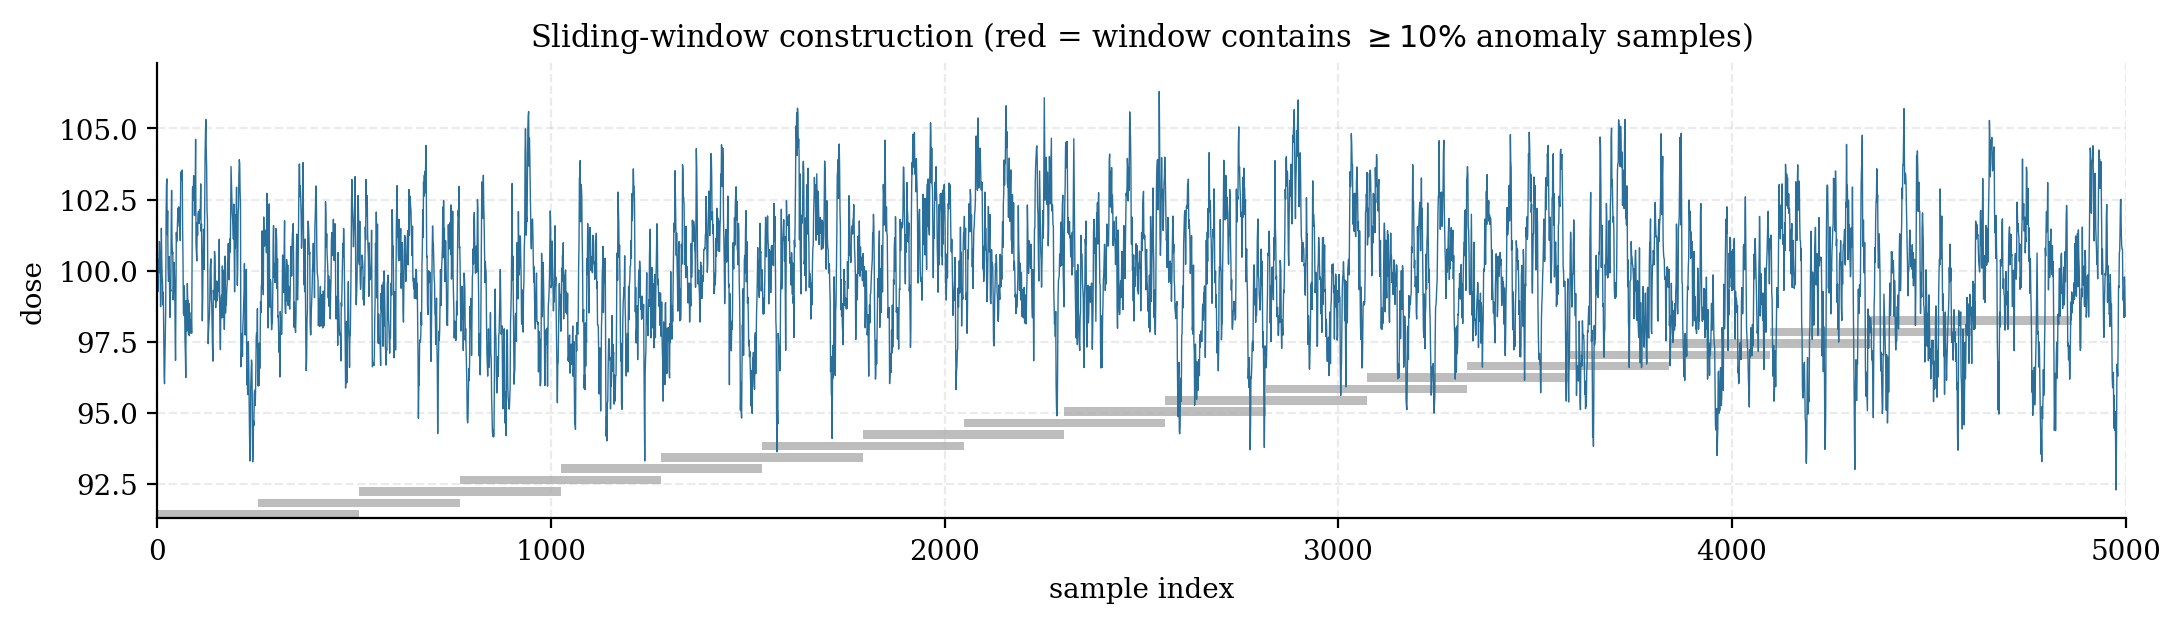
\includegraphics[width=0.92\linewidth]{figures/sliding_window}
    \caption{Sliding-window construction. Each bar is one $512$-sample window;
    a window is labelled anomalous when at least $\tau_{\mathrm{cov}}=10\%$ of its
    samples belong to an event.}
    \label{fig:windowing}
\end{figure}

\paragraph{Per-window normalisation.} Because the baseline drifts, each window is
centred on its own mean and divided by a single global standard deviation
$\sigma_{\mathrm{train}}$ estimated on the centred training windows:
\begin{equation}
    \tilde{\mathbf{x}}^{(t)}
    = \frac{\mathbf{x}^{(t)} - \overline{\mathbf{x}^{(t)}}}{\sigma_{\mathrm{train}}},
    \qquad \sigma_{\mathrm{train}} = 4.21 .
    \label{eq:winnorm}
\end{equation}
The network thus sees only deviations from the local baseline, and the same
$\sigma_{\mathrm{train}}$ is reused at inference.

\section{Building blocks}
\label{sec:blocks}

\paragraph{1D convolution.} The core operator maps a multi-channel sequence
$\mathbf{u}\in\R^{C_{\mathrm{in}}\times L}$ to
$\mathbf{v}\in\R^{C_{\mathrm{out}}\times L'}$ through a learnable kernel of width
$k$:
\begin{equation}
    \mathbf{v}_{c,t}
    = b_c + \sum_{c'=1}^{C_{\mathrm{in}}}\sum_{i=1}^{k}
        \mathbf{w}_{c,c',i}\;\mathbf{u}_{c',\,s\,t+i-p},
    \label{eq:conv}
\end{equation}
with stride $s$ and padding $p$. Weights are shared across time, giving
translation equivariance (an anomaly is recognised wherever it occurs) and a
parameter count $C_{\mathrm{out}}C_{\mathrm{in}}k$ independent of $L$. Each
output channel acts as a learned detector of a local shape. Between convolutions
we apply the pointwise nonlinearity $\ReLU(z)=\max(0,z)$ and reduce resolution
with max-pooling; an \texttt{AdaptiveAvgPool1d(4)} near the end keeps four
temporal bins, retaining a coarse ``where in the window'' cue useful to separate,
e.g., \texttt{fast\_ascend} from \texttt{fast\_descend}.

\paragraph{Normalisation.} Batch normalisation \cite{ioffe2015batch} standardises
each channel over the mini-batch; it is effective but uses running statistics
that differ between train and inference. Group normalisation \cite{wu2018group}
instead normalises over groups of channels \emph{per sample}, so it behaves
identically at train and inference and is amplitude-invariant per window --- a
good match for \cref{eq:winnorm}. We use batch norm in the baseline and group
norm (8 groups) in the two deeper models.

\paragraph{Residual block.} To train depth without vanishing gradients, a
residual block \cite{he2016deep} learns a correction to the identity,
\begin{equation}
    \mathrm{Res}(\mathbf{u}) = \ReLU\!\big(\mathbf{u} + \mathcal{F}(\mathbf{u})\big),
    \label{eq:res}
\end{equation}
where $\mathcal{F}$ is a small Conv--GroupNorm--ReLU stack and a $1{\times}1$
convolution adapts the shortcut when channel counts change.

\paragraph{Self-attention.} For the hybrid model we use a Transformer encoder
\cite{vaswani2017attention}. Given a token sequence $\mathbf{Z}\in\R^{T\times d}$,
attention forms queries, keys and values
$\mathbf{Q},\mathbf{K},\mathbf{V}=\mathbf{Z}\mathbf{W}^{Q},\mathbf{Z}\mathbf{W}^{K},\mathbf{Z}\mathbf{W}^{V}$
and mixes positions by content:
\begin{equation}
    \Attn(\mathbf{Q},\mathbf{K},\mathbf{V})
    = \softmax\!\Big(\tfrac{\mathbf{Q}\mathbf{K}^{\top}}{\sqrt{d_h}}\Big)\,\mathbf{V}.
    \label{eq:attn}
\end{equation}
Several such heads run in parallel (multi-head attention). Unlike a convolution,
one attention layer gives every position access to the whole window, with a
learnt weighting. Since \cref{eq:attn} is order-agnostic, a fixed sinusoidal
positional encoding is added to the tokens; a learnable \texttt{[CLS]} token
\cite{devlin2019bert}, which attends to all others, is read out for
classification.

\section{The three architectures}
\label{sec:arch}

\paragraph{A --- 1D-CNN (baseline).} Three Conv--BatchNorm--ReLU--MaxPool blocks
(kernels $7,7,5$; channels $16\!\to\!32\!\to\!64$), then
\texttt{AdaptiveAvgPool1d(4)} and an MLP head (\cref{tab:cnn}). It is the
simplest model and a sanity check on the pipeline.

\begin{table}[H]
    \centering \footnotesize
    \begin{tabular}{@{}l p{0.5\linewidth} l@{}}
        \toprule
        \textbf{Block} & \textbf{Operation} & \textbf{Output} \\
        \midrule
        Input & raw window & $(1,512)$ \\
        Block 1 & $\Conv(1{\to}16,k{=}7)\,{\to}\,\BN\,{\to}\,\ReLU\,{\to}\,\mathrm{MaxPool}(2)$ & $(16,256)$ \\
        Block 2 & $\Conv(16{\to}32,k{=}7)\,{\to}\,\BN\,{\to}\,\ReLU\,{\to}\,\mathrm{MaxPool}(2)$ & $(32,128)$ \\
        Block 3 & $\Conv(32{\to}64,k{=}5)\,{\to}\,\BN\,{\to}\,\ReLU\,{\to}\,\mathrm{MaxPool}(2)$ & $(64,64)$ \\
        Pool & $\mathrm{AdaptiveAvgPool1d}(4)$ & $(64,4)$ \\
        Head & $\mathrm{Flatten}\,{\to}\,\mathrm{Drop}(0.4)\,{\to}\,\mathrm{Lin}(256{\to}32)\,{\to}\,\ReLU\,{\to}\,\mathrm{Drop}(0.2)\,{\to}\,\mathrm{Lin}(32{\to}K)$ & $(K)$ \\
        \bottomrule
    \end{tabular}
    \caption{Architecture A --- 1D-CNN ($22{,}727$ parameters).}
    \label{tab:cnn}
\end{table}

\paragraph{B --- ResNet 1D.} The same depth, but each block is a residual block
(\cref{eq:res}) with group norm; first-block kernels $(15,9,5)$ for broad
context, then $(7,5,3)$; channels $16\!\to\!32\!\to\!64$ with max-pool between
blocks, then the same pooling and head as model A. Keeping the head identical
makes the residual trunk the only difference from A --- a clean ablation.

\paragraph{C --- CNN+Attention.} A stride-2 convolutional stem (channels
$16\!\to\!32\!\to\!64$, group norm) reduces the length eightfold to $T=64$ tokens
of dimension $d=64$. A learnable \texttt{[CLS]} token is prepended, a sinusoidal
positional encoding added, and two pre-norm Transformer encoder layers
($h=4$ heads, feed-forward width $256$, dropout $0.1$) are applied; the
\texttt{[CLS]} output feeds a linear classifier. The stride-2 stem keeps the
$O(T^2)$ attention cost small.

\begin{table}[H]
    \centering \footnotesize
    \begin{tabular}{lccc}
        \toprule
        & \textbf{1D-CNN} & \textbf{ResNet 1D} & \textbf{CNN+Attention} \\
        \midrule
        Trunk            & 3 plain conv blocks & 3 residual blocks & stride-2 stem + 2 encoders \\
        Normalisation    & BatchNorm           & GroupNorm(8)      & GroupNorm(8) + LayerNorm \\
        Long-range mixing& ---                 & ---               & multi-head self-attention \\
        Parameters       & $22{,}727$          & $74{,}631$        & $109{,}655$ \\
        \bottomrule
    \end{tabular}
    \caption{The three architectures at a glance ($K=7$).}
    \label{tab:arch-compare}
\end{table}

\section{Training}
\label{sec:training}

All models use one recipe (full settings in \cref{app:hp}), implemented in
PyTorch \cite{paszke2019pytorch}. We minimise the class-weighted cross-entropy of
\cref{eq:objective} with Adam \cite{kingma2015adam} (learning rate $10^{-3}$),
batch size $128$, for at most $35$ epochs. The learning rate is halved after two
epochs without validation improvement (\texttt{ReduceLROnPlateau}), and training
stops early after ten such epochs, keeping the lowest-validation-loss weights.
The dataset yields $249{,}985$ training windows (split $80/20$ into train and
validation) and $62{,}485$ test windows. The background class makes up only
$\sim 31\%$ of windows and each anomaly $\sim 11$--$12\%$; the inverse-frequency
weights of \cref{eq:objective} are
$\mathbf{w}=(0.46,1.18,1.27,1.32,1.24,1.15,1.31)$. No data augmentation is used,
as the stochastic generator already supplies variability.
